\documentclass[tikz,border=5pt]{standalone}
\usepackage{amsmath}
\usepackage{pgfplots}
\pgfplotsset{compat=1.18}

\definecolor{racional}{HTML}{365FB3}
\definecolor{quadratica}{HTML}{16803A}
\definecolor{punt}{HTML}{B91C1C}
\definecolor{assimptota}{HTML}{6B7280}

\begin{document}
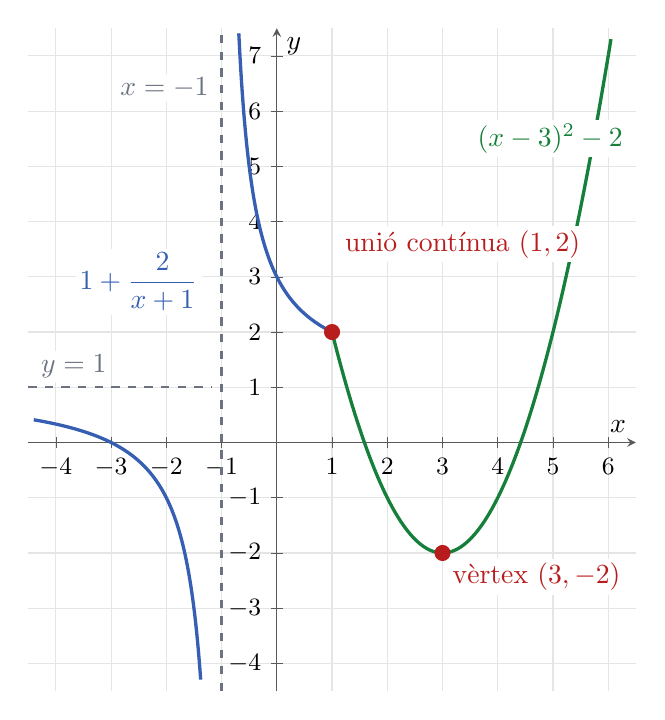
\begin{tikzpicture}
  \begin{axis}[
    width=11.5cm,
    height=10cm,
    axis lines=middle,
    xmin=-4.5,
    xmax=6.5,
    ymin=-4.5,
    ymax=7.5,
    xlabel={$x$},
    ylabel={$y$},
    xtick={-4,-3,-2,-1,0,1,2,3,4,5,6},
    ytick={-4,-3,-2,-1,0,1,2,3,4,5,6,7},
    grid=major,
    grid style={black!10},
    axis line style={black!65},
    tick style={black!65},
    tick label style={font=\small},
    unit vector ratio*=1 1 1,
    clip=true,
  ]
    \addplot[assimptota, dashed, thick] coordinates {(-1,-4.5) (-1,7.5)};
    \addplot[assimptota, dashed, thick, domain=-4.5:-1.18, samples=2] {1};

    \addplot[
      racional,
      very thick,
      domain=-4.4:-1.18,
      samples=180,
      restrict y to domain=-4.5:7.5
    ] {1+2/(x+1)};
    \addplot[
      racional,
      very thick,
      domain=-0.82:0.999,
      samples=180,
      restrict y to domain=-4.5:7.5
    ] {1+2/(x+1)};

    \addplot[
      quadratica,
      very thick,
      domain=1:6.05,
      samples=180
    ] {(x-3)^2-2};

    \addplot[only marks, mark=*, mark size=2.7pt, punt]
      coordinates {(1,2) (3,-2)};

    \node[anchor=south east, text=assimptota, fill=white, inner sep=1.5pt]
      at (axis cs:-1.15,6.15) {$x=-1$};
    \node[anchor=south west, text=assimptota, fill=white, inner sep=1.5pt]
      at (axis cs:-4.35,1.08) {$y=1$};
    \node[anchor=south west, text=punt, fill=white, inner sep=1.5pt]
      at (axis cs:1.15,3.25) {uni\'o cont\'inua $(1,2)$};
    \node[anchor=north west, text=punt, fill=white, inner sep=1.5pt]
      at (axis cs:3.1,-2.1) {v\`ertex $(3,-2)$};
    \node[anchor=south east, text=racional, fill=white, inner sep=1.5pt]
      at (axis cs:-1.35,2.3) {$1+\dfrac{2}{x+1}$};
    \node[anchor=south west, text=quadratica, fill=white, inner sep=1.5pt]
      at (axis cs:3.55,5.15) {$(x-3)^2-2$};
  \end{axis}
\end{tikzpicture}
\end{document}
